One of the main goals of the \Gh\ survey is to explore possibilities of chemical tagging for random field and known open cluster stars. A task that sounds easy in theory, but its working applications are far from ready for large spectroscopic surveys. The road to getting precise stellar chemical abundances leads around many different obstacles, which all have an impact on the final determined abundance values whose precision and accuracy dictates the possibility and success of implementing chemical tagging.

In this chapter, we present our exploration of abundances for a few open clusters that were observed as part of multiple different surveys served by the HERMES spectrograph. In Section \ref{sec:intro_tag}, we briefly describe the history of open cluster membership, the evolution of clusters, and means to discover these ongoing processes using stellar abundance information only. Of multiple observed open cluster in the GALAH, we focus only on a small subset of them that have the highest number of members (see Section \ref{sec:galah_clusters} for the complete list). Section \ref{sec:membership_v2} describes the selection of clusters and integration of orbits for stars inside and around the clusters. Chemical signature of field and cluster stars is analysed in Section \ref{sec:chem_ej_tag} and the results are summarised and discussed at the end of this chapter.

\section{Introduction}
\label{sec:intro_tag}
The latest second release of \G\ data (\Gs, \cite{2018A&A...616A...1G}) revolutionized numerous fields of astronomy, including research of galactic open clusters. Its combined information of stellar distance, kinematics, and photometric measurements enables us to go beyond simple methodologies, such as star density counts, to unravel even the faintest and sparsest components of open clusters. So far, many works have been published trying to refine parameters, and membership information of long known open clusters \cite{2017A&A...601A..19G, 2018A&A...618A..93C, 2019A&A...627A..35C} and find new, less numerous or fainter clusters \cite{2019ApJS..245...32L, 2019JKAS...52..145S, 2019A&A...624A.126C, 2020arXiv200107122C}. Such thorough and the improved investigation uncovered that many of the clusters listed in modern catalogues, initially discovered as apparent stellar overdensities, are no more than chance alignments of stars and not true physical clusters \cite{1998A&A...340..402B, 2000A&A...357..145C, 2016AJ....152....7H, 2018MNRAS.480.5242K, 2020A&A...633A..99C}.

Born from the same molecular cloud, open clusters are ideal test structures for different astrophysical principles. Being influenced by external and internal processes, such as tidal stripping and close stellar interactions, their lifetime is limited from about 100 Myr to a few Gyr for the densest structures \cite{1998A&A...337..363P, 2013MNRAS.434.2509M}. This gives us a possibility of observing them at different evolutionary stages \cite{2006BASI...34..153C, 2007A&A...468..139P} before they blend \cite{2001A&A...366..827B} into field stellar population. The most prominent transitional features we can observe are compact cluster tidal tails \cite{2019AA...627A...4R, 2019AJ....157..115Y, 2019AA...621L...3M, 2019arXiv191206657Z} and lose extended halos of evaporated stars. They are observed as a slowly decreasing over-density \cite{2002A&A...385..471C, 2004A&A...427..485B, 2019AA...627A.119C} of stars far from a denser cluster core. Due to close gravitational interactions among members, they can be ejected out of a cluster at high velocities \cite{2009MNRAS.396..570G, 2010MNRAS.402..105G, 2017MNRAS.470.3049R}. Such cluster members can on the sky be found several degrees or even further away from their main cluster body \cite{2007MNRAS.376L..29G, 2018MNRAS.473.4612K, 2019ApJ...884....6M}. Identification of such stars could be done using a chemical tagging procedure, whose importance and potential problems have already been discuses in Section \ref{sec:open_clustesr_tagging}. 

\section{Additional data specifics}
\label{sec:data_clusters}

\subsection{The GALAH and cluster stars}
\label{sec:galah_clusters}
Among the dedicated HERMES cluster observations and other HERMES surveys, such as the main \Gh\ survey, we detected members of known open clusters, whose stellar membership was taken from results published by \citet{2018A&A...618A..93C}. Their clustering methodology relies on the unsupervised membership assignment code called Unsupervised Photometric Membership Assignment in Stellar Clusters (UPMASK, \cite{2014A&A...561A..57K}). Initially, the methodology was designed to find overdensities using only stellar position and photometry. As the methodology is unsupervised and has zero knowledge about physics or input data, \citet{2014A&A...561A..57K} easily applied it to work with astrometric and positional data. Internally UPMASK creates many incarnations of random values from the input data and their uncertainties, selects the four most important principal components, and runs the clustering algorithm on the components. At the end, detected overdensities are compared with random stellar fields and overdensities of the last iteration. Membership probabilities depend on how often a star was inside the relevant overdensity.

As some of the clusters were not targeted intentionally by the surveys or only their cores, the number of observed members and surrounding field stars of interest can vary substantially. The clusters analysed in this paper, having the most significant number of spectroscopic observations are Berkeley 32, NGC 2516, NGC 2112, NGC 6253, Blanco 1, Ruprecht 147, NGC 2632, NGC 2682,  Melotte 22, and Collinder 261. To supplement their selection, we added members of Melotte 25 cluster whose membership selection was performed by us as it was missing in the mentioned published paper \cite{2018A&A...618A..93C}. The first step of our methodology was comparable to UPMASK. Similarly, we generated many incarnations of the data to determine the kinematics of a cluster. It was computed as a median proper motion of the over-density that was closest to the previously known centre at every iteration. After selection in proper motion space, we used the same stars to determine clusters centre in position, distance, and radial velocity. A multivariate Gaussian distribution was fitted at the determined parameter to assess membership probabilities.

\subsection{Gaia}
\label{sec:gaia_clusters}
For a complete 6D positional and kinematics stellar information, we augmented the \Gh\ data with proper motion, parallax and radial velocity from the \Gs\ data-set. As all investigated open cluster stars are located close to the Sun, their distances can be inferred by the inversion of a parallax value ($1 / \varpi$). Of course, we could, at this point, use a bit more accurate distances that were determined using distance priors based on a Galaxy model \cite{2018AJ....156...58B}. The second approach does give more reliable and symmetric distance uncertainties, but does not reduce the elongated shape of stellar clusters (in radial direction away from our location in the Galaxy) as the distance to every star is determined individually. At the same time, more distant stars have grater relative parallax uncertainties which makes it even more difficult to determine distance and shape of a cluster. To get a more realistic shape of a cluster, all member distances would have to analysed at the same time with inclusion of the isochrone information.

The current release of the \G\ data contains magnitude limited range of recovered radial velocities, that are, whenever possible, supplemented or substituted with the \Gh\ measurements of higher accuracy \cite{2018arXiv180406344Z}. Supplemented are mostly stars fainter than currently adopted \G\ RVS \cite{2018A&A...616A...5C} analysis threshold as the GALAH targets are much fainter stars than the RVS limit. The synergy, therefore, increases the set of useful stars in our case.

\section{Cluster and field members}
\label{sec:membership_v2}
The first step in our analysis was the acquisition of data relevant for each cluster identified among the \Gh\ observations. Identification of observed clusters was made by matching observed stars with known cluster members published by \citet{2018A&A...618A..93C}. As some of the clusters had a low number of stars or were proved to be chance alignments of stars \cite{2018MNRAS.480.5242K}, they were not considered in the analysis. Sky coordinates and distances of selected open cluster members (see Section \ref{sec:galah_clusters} for the list of considered clusters) were taken from \citet{2018A&A...618A..93C} and served us as anchors around which we queried the \Gs\ data. A cone query with a radius of $6^\circ$ and distance limit of $\pm900$~pc around a cluster centre was performed to download a subset of the whole dataset. The elongated shape of queried dataset volume is a result of clusters' apparent elongated shape. A bit different volume was used for a nearby and visually extensive cluster Melotte 25, for which we used radius of $12^\circ$ and distance limit of $\pm200$~pc around its centre. 

The downloaded subset included stars with an incomplete set of \G\ parameters. To complement and improve quality of radial velocity measurements, all available \Gh\ velocity estimates in a subset were used to override or supplement \G\ measurements. In the case of multiple \Gh\ observations, a median velocity per star was used. 

The initial open cluster memberships were taken from \citet{2018A&A...618A..93C} but needed some refinement before it was suitable for us. To select as many possible cluster members, the employed membership algorithm did not relay on magnitude limited radial velocity information to assign cluster membership. To make cluster volume more compact and retain only the most probable core members, we discarded all member stars whose radial velocity deviated for more than $5$~\kms\ from the cluster median value of all retrieved members. The used threshold was determined empirically by observing velocity distributions to discard only a few of the most dissimilar stars. The reason behind this velocity limitation will be evident in Section \ref{sec:orbit_tracing} where we try to keep the cluster volume as compact as possible during its integration. This thresholding prevents unwanted pollution of a cluster by field stars during comparison of their chemical signatures in Section \ref{sec:chem_cluster}. 

\subsection{Stellar tracing}
\label{sec:orbit_tracing}
After the selection of open cluster members, we proceeded with the analysis of stellar movements inside and outside the cluster. In order to get the most reliable motion information, only stars with a complete 6D kinematic information (proper motion + radial velocity + sky coordinate + parallax) were considered. No additional \G\ quality flagging was used to remove stars with potentially wrong parameter estimates as we would like to show in the following steps that they could be discovered and eliminated based solely on their chemical composition.

By knowing members of the observed clusters, their current position, and complete motion vectors, we can trace the path of a volume constrained by the cluster stars backwards or forwards in time. This integration procedure was performed by individual integration of cluster stars in axisymmetric gravitational potential (\textit{MWPotential2014} potential described by \citet{2015ApJS..216...29B}) using \GP\ software library version 1.5.0. \cite{2015ApJS..216...29B}. Being interested in the past ejected members of a cluster, we integrated orbits of cluster stars for $120$~Myr (comparable to ages of the youngest open clusters in our set) into their past and saved their location after every step of $20$~kyr. As the integration process relies only on the present uncertain measurements of their velocities and distance, longer integration is not precise or reliable. This uncertainty is observed by the fact that the cluster volume gets larger during backwards integration instead of staying approximately constant as it would in the case of gravitationally bound stellar components. The volume could also keep shrinking during backwards integration if cluster is loosely bound and is already slowly dissipating at the present time. At every integration step, the cluster volume was described by a minimum convex hull defined by its outer-most members. They serve as vertex points of the constructed geometric body. Such a geometrical shape presents the smallest bounding volume with partially flat boundaries which encompasses all considered members.

The next step of our analysis consisted of finding stars in the clusters' immediate neighbourhood that could be traced back to having origin inside the considered open cluster. To filter-out field stars that travel into a completely different direction than the cluster, we discarded all stars whose galactic velocity vector difference towards present cluster velocity vector was >$50$~\kms. This threshold, therefore, defines the fastest possible speed at which stars could have been ejected. Orbits of the remaining set of stars (usually more than half of the queried stars) were integrated using the same configuration as cluster stars described above. At this point, we could investigate which orbit of the field stars crosses clusters' volume at any given integration step.

To get a more descriptive crossing probability, we created $250$ incarnations of every field star. Initial kinematic properties of each incarnation were drawn from the Gaussian distributions of parallax, radial velocity, and proper motion defined by their reported values and uncertainties. After analysing all $250$ orbits of each star, we described its cluster crossing probability by the longest stay inside the cluster volume and  by the percentage of crossing events. For a crossing to be counted as confirmed, a star had to be located inside the cluster volume for at least $0.4$~Myr -- time that is equivalent to $20$ integration steps. The final selection of probable ejected stars consist of stars, whose integration procedure revealed that they were crossing a cluster volume in at least $68$\% of the incarnations and their longest stay there was at least $1$~Myr. Remaining volume crossing stars, that did not meet the criteria, were considered as random field stars. They were also discarded from further analysis as they might, in the case they were real past cluster members, additionally pollute chemical signature of the field population. Summary of investigated and discovered stars for every cluster is given in Table \ref{tab:cluster_stats}.

\begin{table}
	\centering
	\caption{Clusters statistics. Only stars with a complete 6D positional and kinematic information were considered for this statistics and orbit integration analysis. Numbers in columns successively present: number of all stars with complete information, number of analysed stars that meet initial criteria of having the galactic velocity similar to a cluster ($\Delta$v~<~50~\kms), number of stars that do not cross cluster volume during integration, number of possibly ejected stars, and number of cluster members that defined volume of a cluster.}
	\begin{tabular}{l c c c c c }
		\hline
		Cluster & Queried from & Analysed & Field & Possibly & Known \\
		 & \G\ DR2 & stars & stars & ejected & members \\
		\hline \hline
		Berkeley 32  & 11322 & 2659 & 2047 & 125 & 23 \\ 
		Blanco 1     & 5043 & 2734 & 2687 & 15 & 81 \\
		IC 4665      & 15022 & 10155 & 9823 & 26 & 34 \\
		Mamajek 4    & 21776 & 11623 & 10513 & 85 & 48 \\
		Melotte 22   & 9097 & 6335 & 5944 & 105 & 239 \\
		Melotte 25   & 6836 & 3782 & 3511 & 165 & 126 \\
		NGC 1817     & 12826 & 4489 & 4060 & 74 & 54 \\
		NGC 1901     & 12666 & 7323 & 7204 & 19 & 30 \\
		NGC 2112     & 13866 & 6665 & 6323 & 38 & 49 \\
		NGC 2204     & 4314 & 1777 & 1170 & 180 & 59 \\
		NGC 2516     & 17383 & 11906 & 11030 & 315 & 182 \\
		NGC 2548     & 14371 & 9212 & 8842 & 60 & 34 \\
		NGC 2632     & 9951 & 5290 & 4991 & 170 & 222 \\
		NGC 2682     & 10947 & 5244 & 4776 & 226 & 287 \\
		NGC 6253     & 62975 & 30114 & 17267 & 1362 & 64 \\
		Ruprecht 147 & 17749 & 5062 & 4850 & 23 & 103 \\
		\hline
	\end{tabular}
	\label{tab:cluster_stats}
\end{table}

\section{Chemical signature of clusters}
\label{sec:chem_cluster}
After defining potential members of different cluster components (field, ejected, and members), we can look into the abundance signatures of an individual component and their overlap. Of all 30 possible \Gh\ chemical abundances, we initially excluded only Li because of its intrinsic variability that depends on the stellar evolutionary stage. Scatters plots of all considered abundances and \Feh\ as a function of \Teff\ for clusters most populated by the \Gh\ data are shown in Figures \ref{fig:ct_cluster1}, \ref{fig:ct_cluster2}, \ref{fig:ct_cluster3}, and \ref{fig:ct_cluster4}. Not all plots for the same cluster have the equal number of points as reporting of abundance values depends on the estimation of their reliable detectability that is based on equivalent widths of elemental absorption lines (thoroughly described in \citet{buder2020}). The plots show only stars with unflagged (\texttt{flag\_sp} = 0, other flag values are described in \citet{buder2020}) stellar parameters, that are presumably of the highest quality.

\begin{figure}
	\centering
	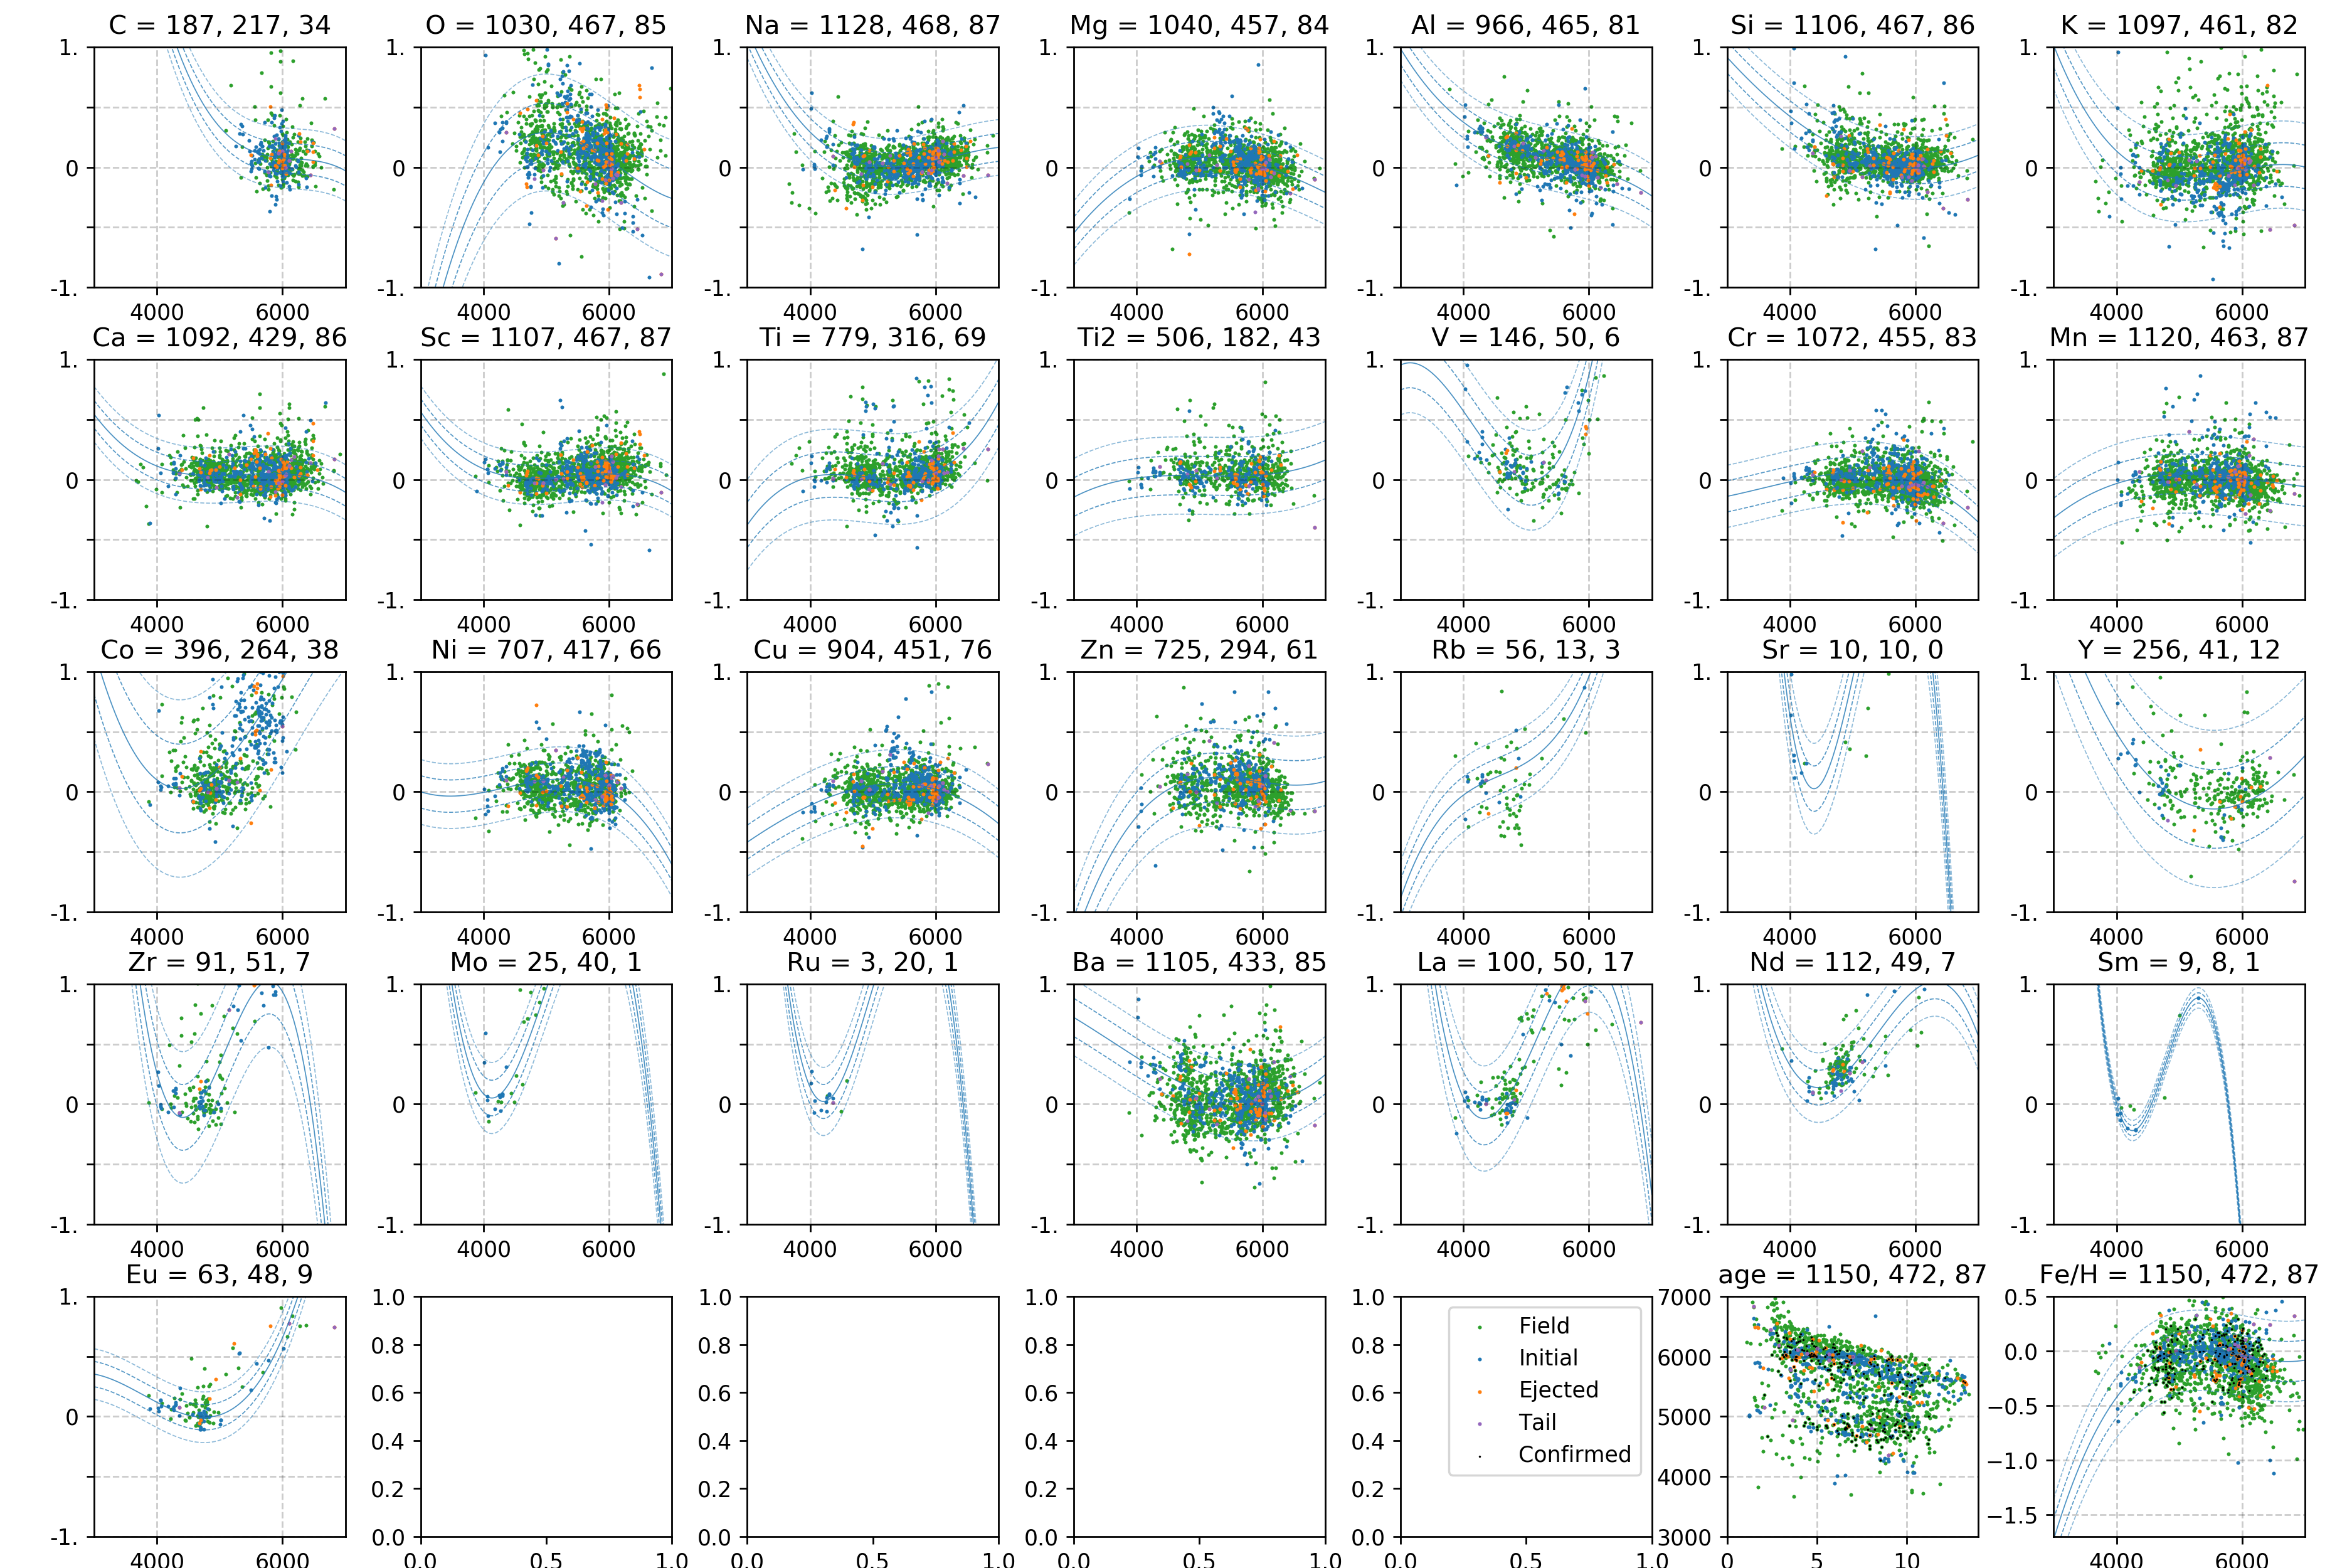
\includegraphics[width=\textwidth]{p_teff_abundances_NGC_2682_orbits_DR3_new_flag0.png}
	\caption{NGC 2632 abundance scatter plots as a function of effective stellar temperature. The solid blue line represents the best fit on the cluster population. The 1$\sigma$ and 2$\sigma$ abundance deviations from the fit are given by dashed blue lines of decreasing intensity. Coloured dots represent field (green), members (blue), and possibly ejected (orange) stars. Their numbers are given above every panel, following the elements' name. Purple dots preset known tails (described later in Section \ref{sec:tails_chem}) of slowly evaporating stars in some clusters. The last two panels present \Teff\ of stars at different ages (in Gyr), and dependence of \Feh\ on their \Teff. The black dots in those two panels indicate possibly ejected stars whose chemistry was matched to cluster stars.}
	\label{fig:ct_cluster1}
\end{figure}

\begin{figure}
	\centering
	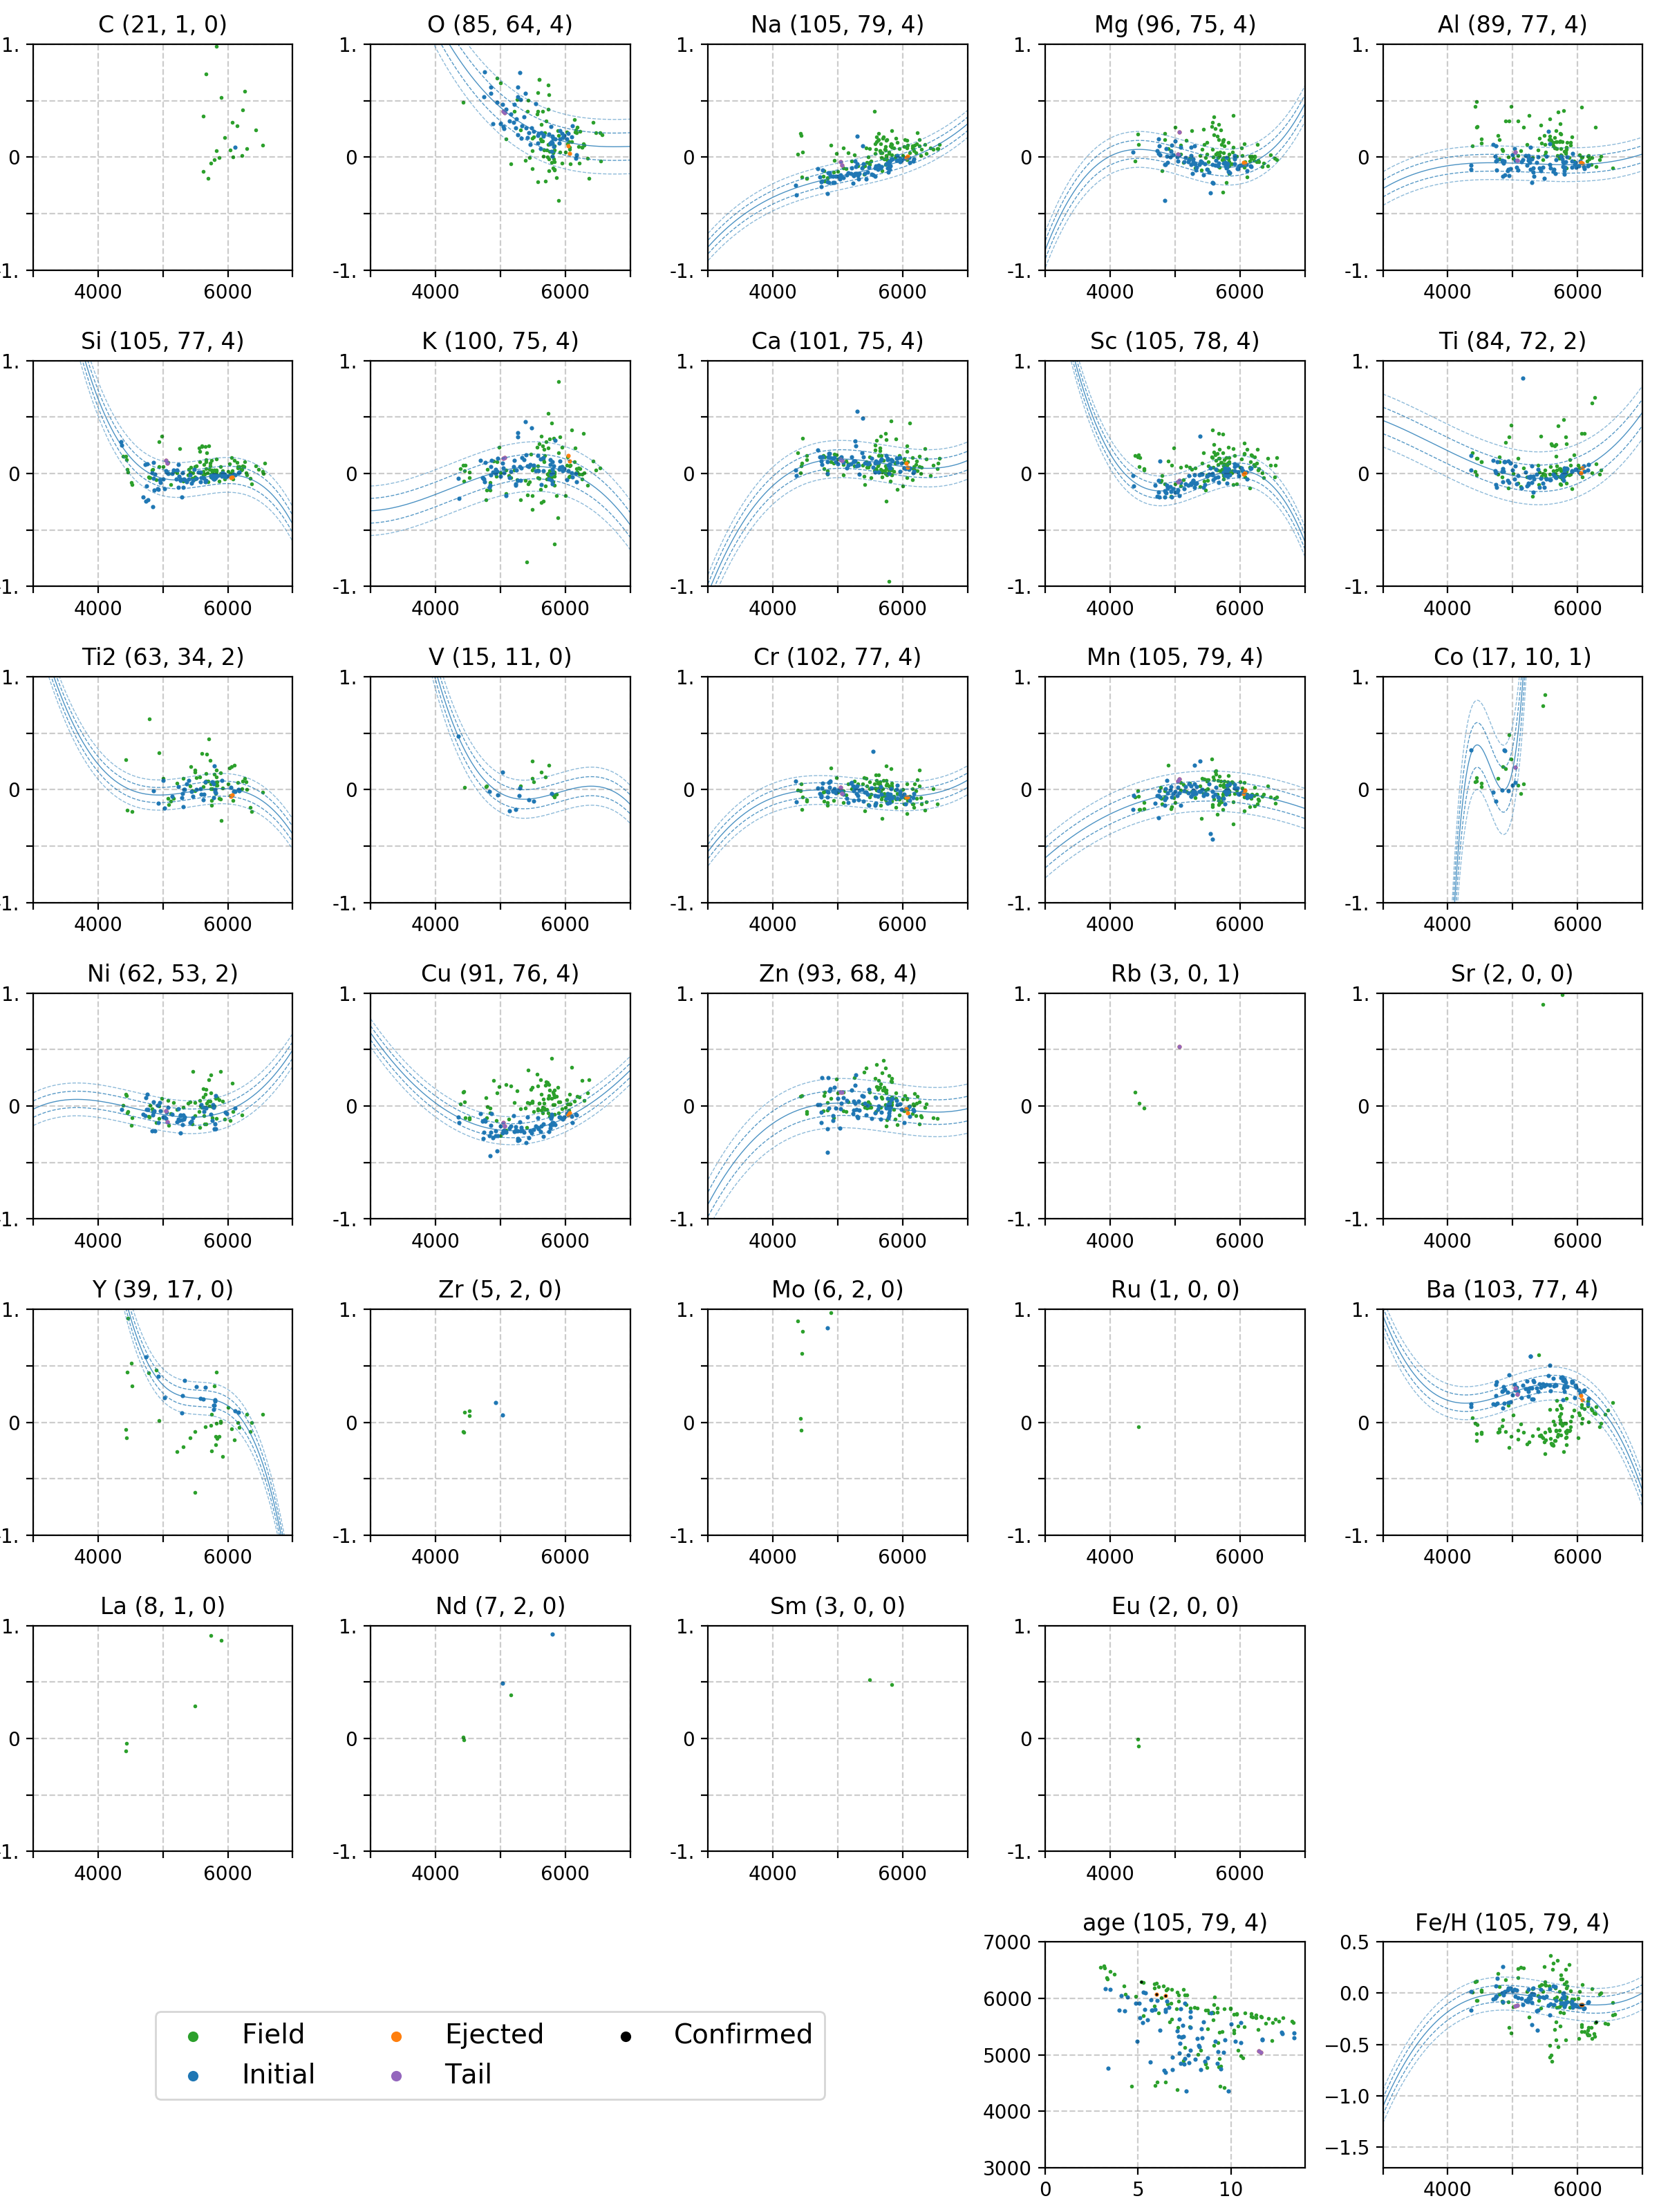
\includegraphics[width=\textwidth]{p_teff_abundances_Blanco_1_orbits_DR3_new_flag0.png}
	\caption{Same plots as in Figure \ref{fig:ct_cluster1} but for open cluster Blanco 1.}
	\label{fig:ct_cluster2}
\end{figure}

\begin{figure}
	\centering
	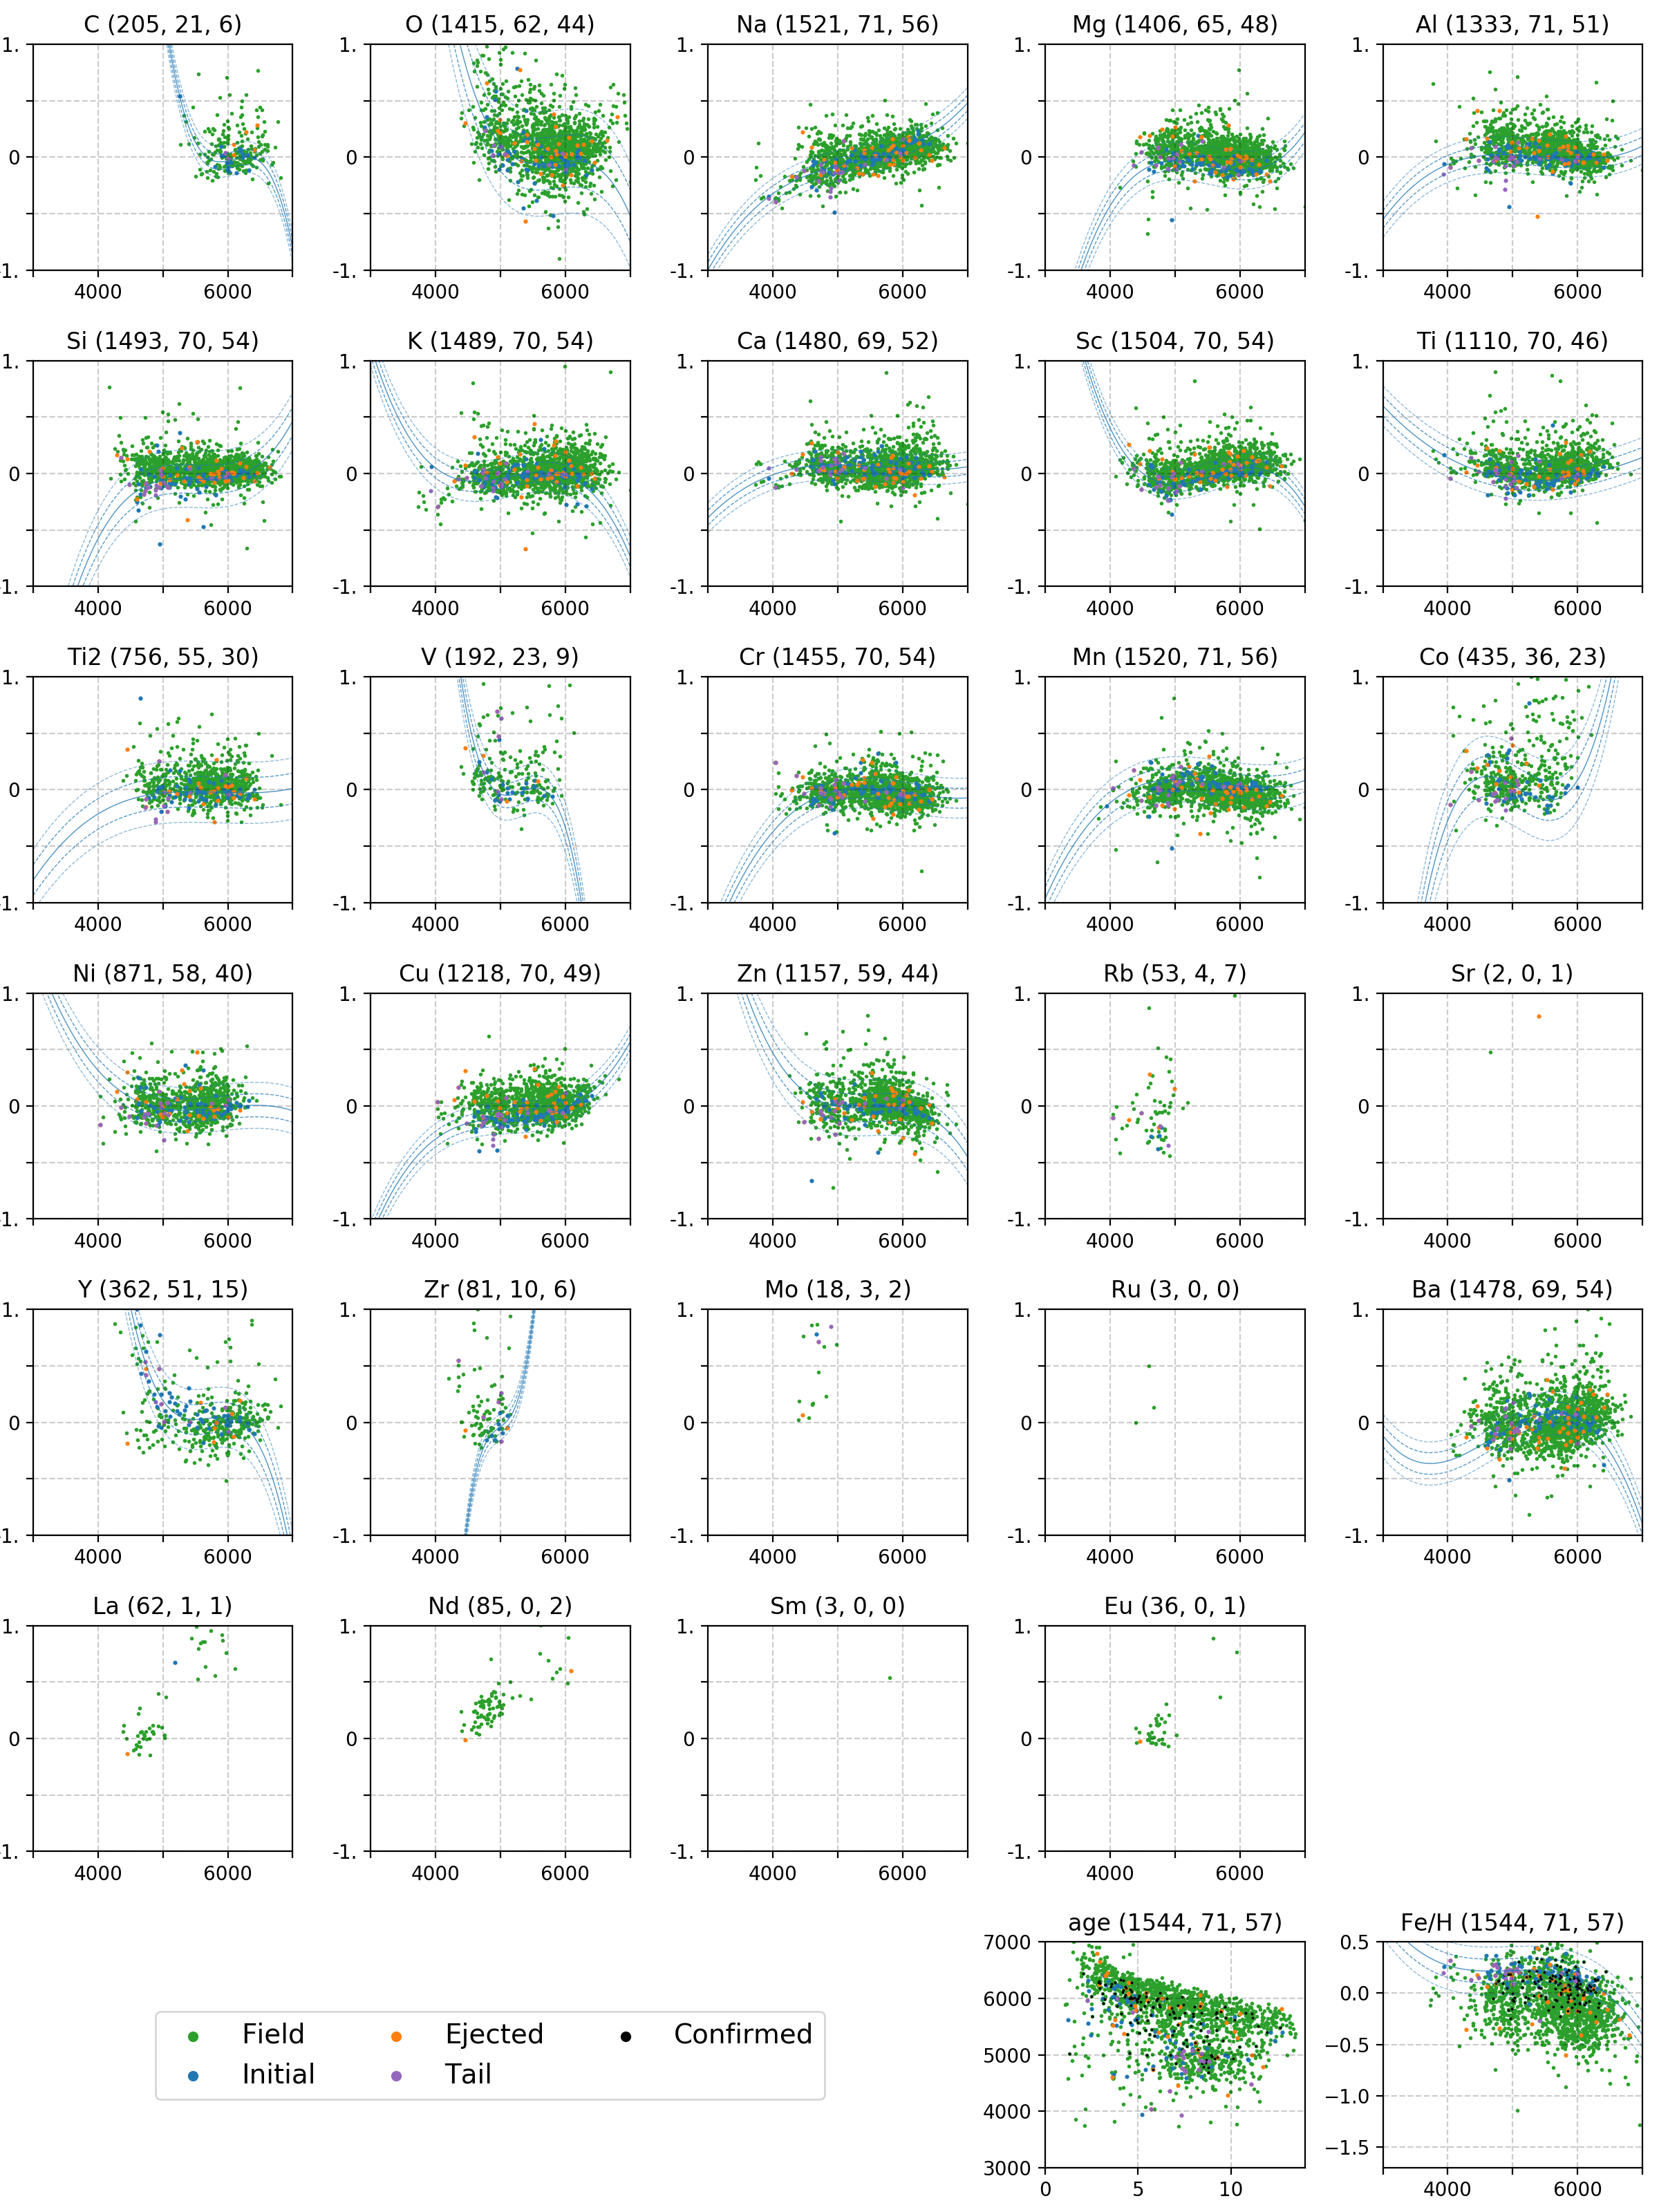
\includegraphics[width=\textwidth]{p_teff_abundances_NGC_2632_orbits_DR3_new_flag0.png}
	\caption{Same plots as in Figure \ref{fig:ct_cluster1} but for open cluster NGC 2632.}
	\label{fig:ct_cluster3}
\end{figure}

\begin{figure}
	\centering
	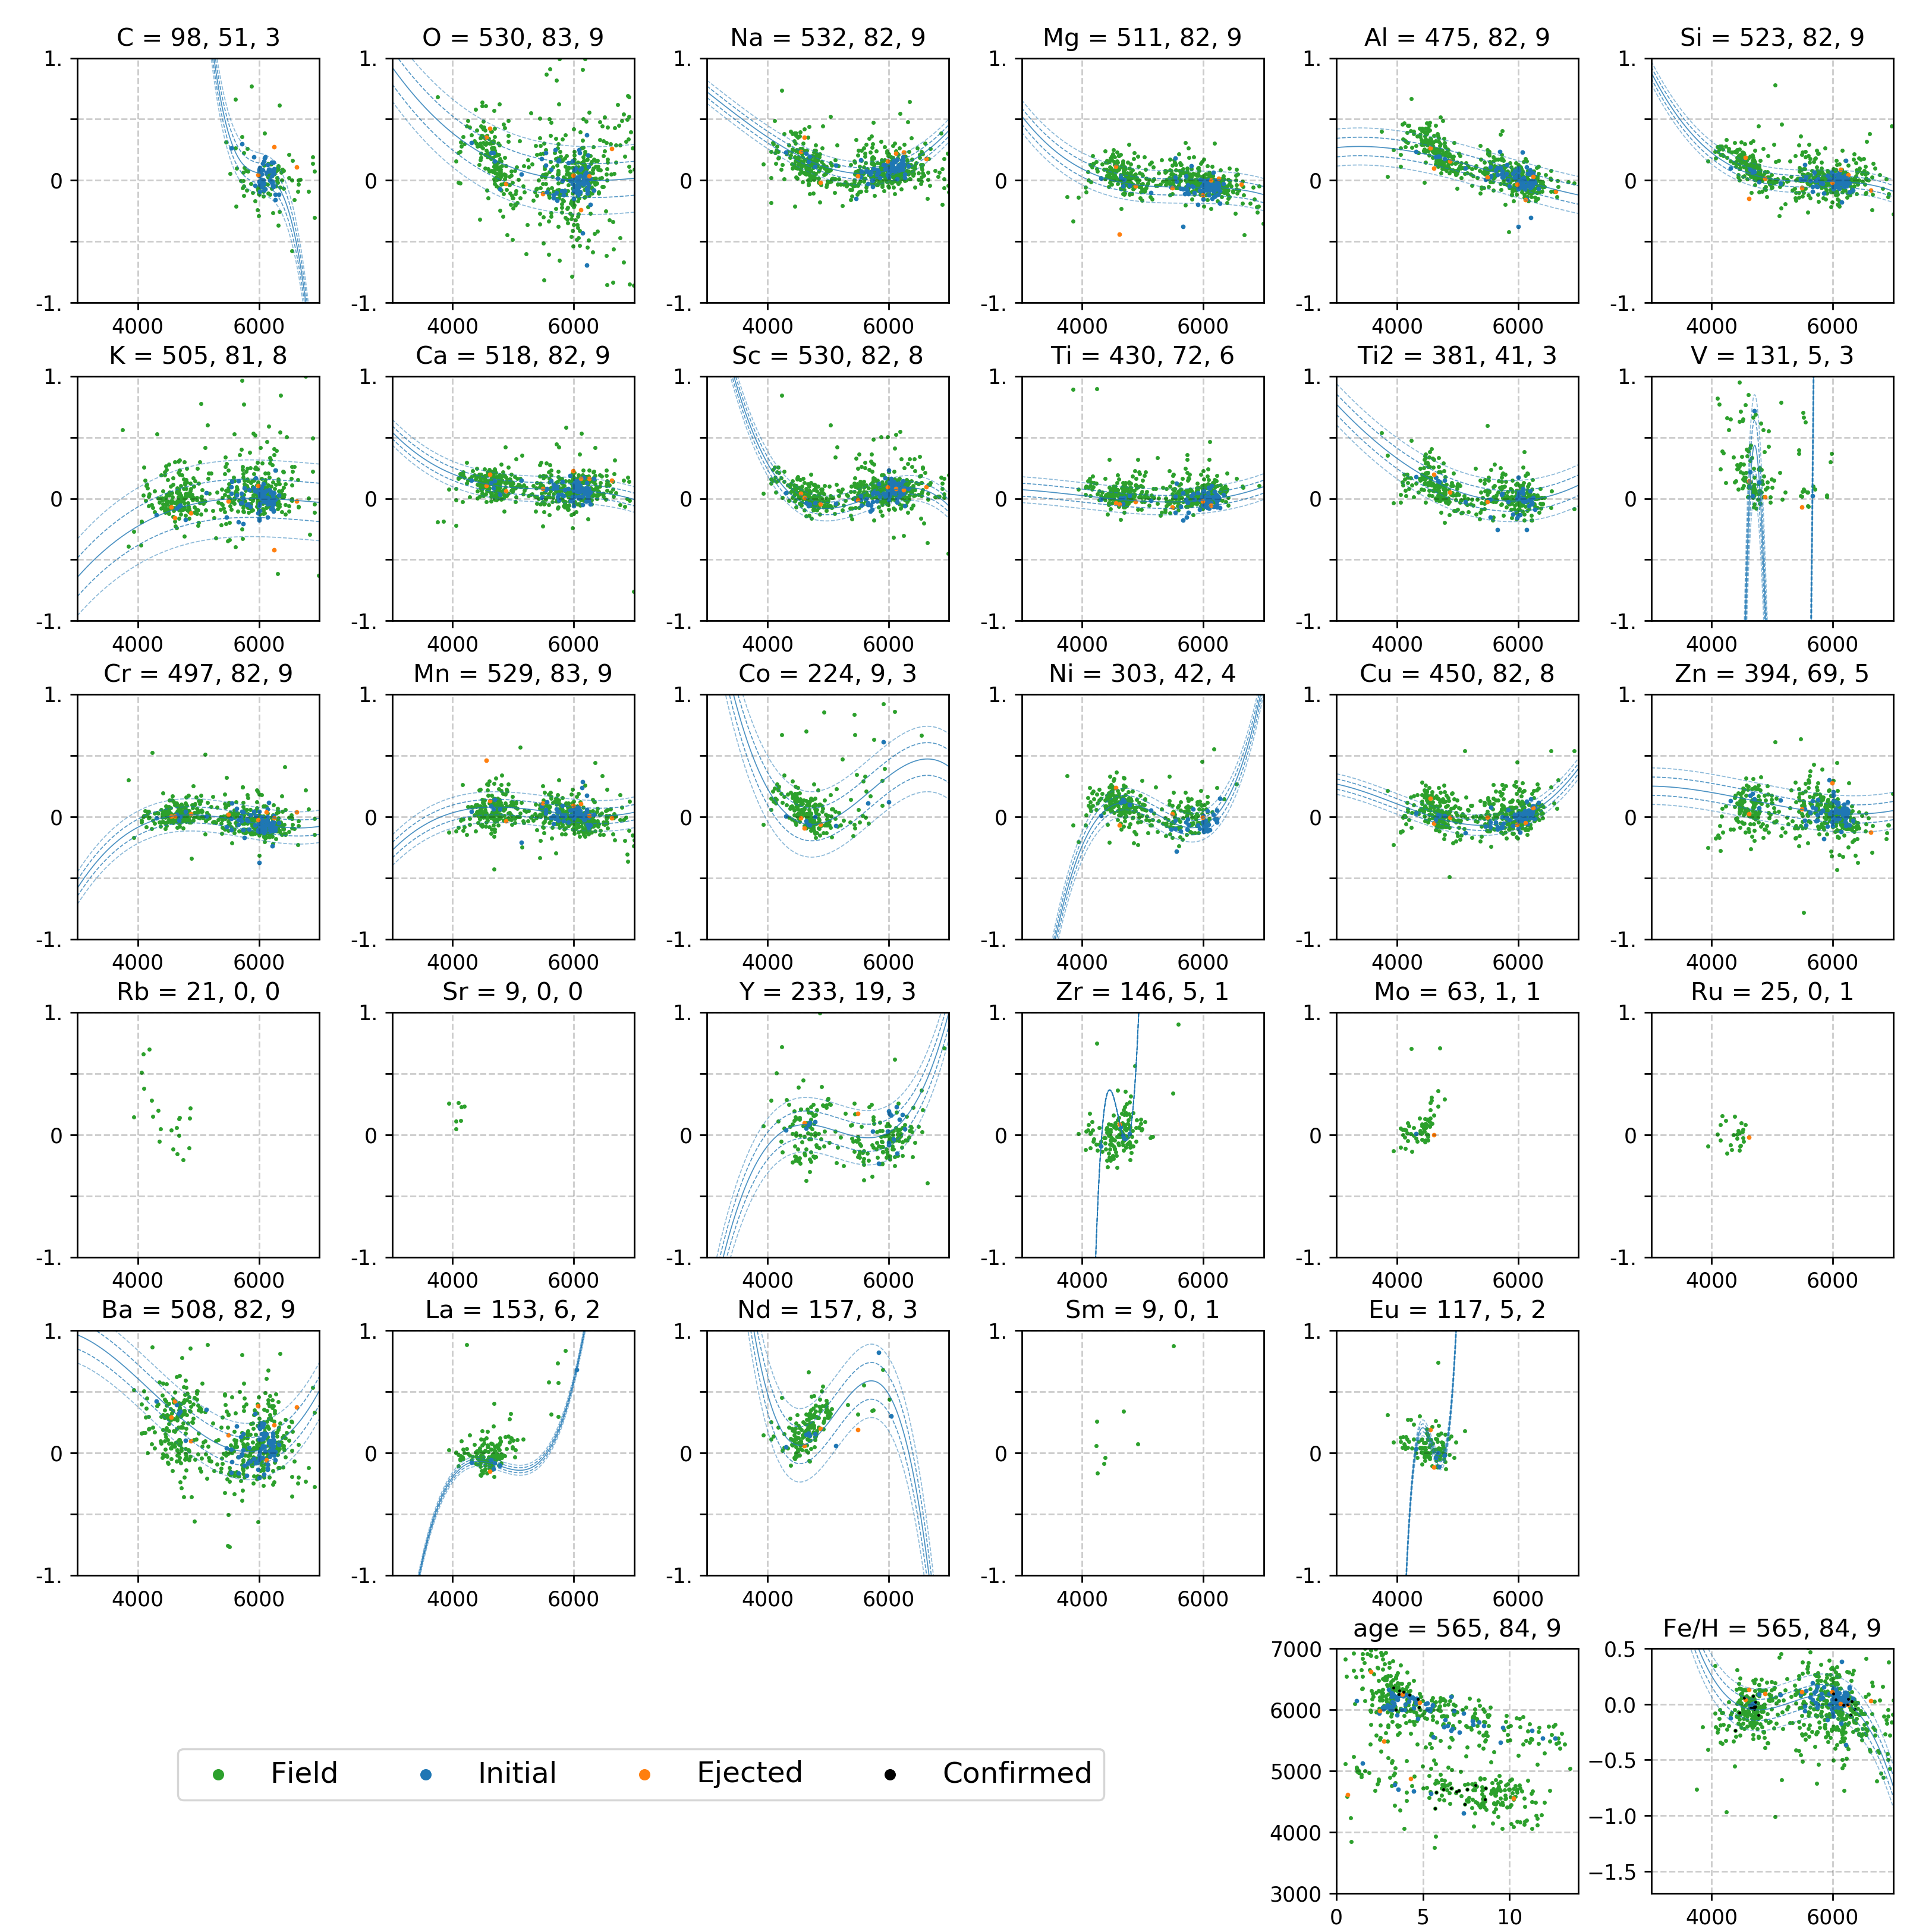
\includegraphics[width=\textwidth]{p_teff_abundances_Ruprecht_147_orbits_DR3_new_flag0.png}
	\caption{Same plots as in Figure \ref{fig:ct_cluster1} but for open cluster Ruprecht 147.}
	\label{fig:ct_cluster4}
\end{figure}

\begin{table}
	\centering
	\caption{The number of acquired \Gh\ spectra among different cluster components that were considered during the chemical comparison. No parameter or abundance flagging was yet used at this point. Stars represented by these statistics are a subset of stars given in Table \ref{tab:cluster_stats}. Because of a small percentage of repeated observations, few clusters (especially NGC 2682 that was used as the calibration and verification field) can have a higher number of spectra than the number of member stars.}
	\begin{tabular}{l c c c }
		\hline
		Cluster & Field & Ejected & Members \\
		\hline \hline
		Berkeley 32  & 42 & 2 & 36 \\ 
		Blanco 1     & 151 & 10 & 109 \\
		IC 4665      & 1114 & 6 & 26 \\
		Mamajek 4    & 2907 & 26 & 13 \\
		Melotte 22   & 1016 & 21 & 67 \\
		Melotte 25   & 653 & 27 & 64 \\
		NGC 1817     & 569 & 11 & 36 \\
		NGC 1901     & 6963 & 19 & 28 \\
		NGC 2112     & 401 & 4 & 66 \\
		NGC 2204     & 129 & 23 & 58 \\
		NGC 2516     & 4604 & 101 & 48 \\
		NGC 2548     & 767 & 6 & 18 \\
		NGC 2632     & 2266 & 77 & 116 \\
		NGC 2682     & 1710 & 147 & 1000 \\
		NGC 6253     & 825 & 34 & 86 \\
		Ruprecht 147 & 798 & 14 & 175 \\
		\hline
	\end{tabular}
	\label{tab:cluster_stats_abund}
\end{table}

\subsection{Abundance and age trends}
\label{sec:abund_trends}
%Ker vidimo in tudi drugi modeli kar mocne trende zastopanosti v odvisnosti od fizikalnih parametrov zvezd, je treba te nekako spraviti na isto raven. Najlazje diferencialno - naredimo fit na kopico in gledamo koliko ostali odstopajo od tega
One of the first things we noticed on the shown abundance scatter plots is their strong dependence on physical parameters, especially \Teff. As this is not the first or unique observation of those trends \cite{2010A&A...523A..71G, 2013ApJ...775...58B, 2016MNRAS.457.3934L, 2018A&A...619A.176B, 2019arXiv191208539C}, they are most likely products of insufficient/inaccurate stellar models and/or actual abundance patterns, and not induced solemnly by the employed \SME\ spectrum analysis pipeline that was used by \citet{buder2020} to determine stellar abundances.

If we presume that observed trends are artificially induced and considered cluster members should have a homogeneous chemical composition that is independent of stellar type, a differential chemical tagging analysis can be used \cite{2019arXiv191208539C}. Such analysis considers only comparisons among stars with a similar set of stellar parameters. To describe observed trends, we independently fitted a 3$^{rd}$ degree polynomial function using $2.5\sigma$ clipping algorithm in 2 steps to every abundance versus \Teff\ diagram. By subtracting fitted trends, we estimated degree of intracluster scatter for every element. Because of limitations of measuring certain abundances, the fit was not performed if the number of valid abundance measurements was lower or equal to a used polynomial degree $+1$.

In the ideal case, all of the trends for the same element observed in different open clusters would have the same shape and would be distinguished only by their abundance offsets that result from their distinct chemical pattern. Looking at our fitted trends, everything is not so simple and easy as the fitted curves can have significantly different shapes. For example, trends of elements Ba and Cu are in general U-shaped. Therefore the highest or lowest abundance values are present in the middle of the \Teff\ region. Those results imply that using the latest \Gh\ abundances, we can not easily find the global behaviour of measured elements. Blindly using the wrong trend line would, therefore completely change results in our case.

Additional identification that there might something be wrong with the parameters lies in the determined ages of individual stars in the clusters. The ages are determined by the best fitting isochrone with appropriate stellar \Feh\ that lies closest to the stars' position on H-R diagram (further details in \citet{buder2020}). As the procedure is run independently for every star in the survey, ages among cluster stars (see plots in Figures \ref{fig:ct_cluster1}, \ref{fig:ct_cluster2}, \ref{fig:ct_cluster3}, and \ref{fig:ct_cluster4}) are strewn over a range of 5~Gyr or more. Fortunately the abundance computation does not require information about the stellar age, but they both share the requirement for an accurate information about the basic stellar parameters.

% TODO Fino bi bilo (morda tudi na grafu) nekako označiti privzeto starost te kopice. Starost ima gotovo tudi precejšnje napake - najbrž je najbolj točna za MSTO (če jih imaš že kaj), pa morda tudi za hladne, ki se šele usedajo na MS. Komentarji tega tipa sodijo v glavni tekst, tu le omeniš, da so tam.

\subsection{Determining chemical similarity}
\label{sec:chem_ej_tag}
%Pogledamo trende in fite, ter koliko moznih izvzenih zvezd se poraja in sklada s temi kemicnimi trendi. Morda nek threshold koliko je dobrih oziroma skladnih s samo kopico, saj ima tudi ta le kar nekaj razpona v izmerjenih/izracunanih vrednostih parametrov.
Having an analytical description of an individual abundance behaviour for every cluster, we can estimate how many and how accurately do the identified ejected stars match with cluster abundance patterns and trends. The most straightforward way to perform this is to count how often does abundance value of an investigated star fall inside a $1\sigma$ (or $2\sigma$ for a more relaxed selection) region around an abundance trend. Both regions and fitted trends are visualised in Figures \ref{fig:ct_cluster1}, \ref{fig:ct_cluster2}, \ref{fig:ct_cluster3}, and \ref{fig:ct_cluster4}. Before performing such counting, we additionally omitted abundance trends of the following chemical elements: V, Rb, Sr, Y, Zr, Mo, Ru, La, and Sm. Their low number of successful measurements per cluster and uncertain trends were not beneficial to the whole chemical tagging experiment and influenced only a small fraction of stars. In general it is not advised to reduce the dimensionality of chemical space for greater differentiation between chemical signatures. As this was one of the first experiments analysing whether the latest \Gh\ DR3 abundances could be used for cluster and global blind tagging, we tried to remove as many additional systematic effects of uncertain measurements as possible. In our case, an individual star was counted as chemically similar if it matched (e.g. fell inside selected $\sigma$ region around the fitted trend line) to a cluster in at least $68$\% of the considered abundances with valid trend fit. Chemically similarity of ejected stars, given as percentage of tagged stars, is presented in Table \ref{tab:cluster_stats_abundtag}.

% TODO To je ok za tabelo 3.3. Morda pa bi v diskusiji tabele 3.3 bilo smiselno pogledati, kako se obnašajo posamezni elementi, recimo ali so še kakšni poleg V, Rb, Sr,... ki zganjajo probleme. Morda tudi, v katere skupine sodijo: a se recimo vsi slow-r elementi obnašajo podobno ali ne. Če se odločiš iti po tej poti, je potem to o različnih kanalih nastajanja elementov dati v uvodna poglavja.

\subsection{Tagging remaining field stars}
\label{sec:chem_fi_tag}
%Kaj se zgodi ce iste kemicne informacije in thresholde uporabimo se za ostale analizirane zvezde v bljizini. Dobimo sploh kaj zvezd ven iz tega in kaksen bi bil v tem primeru njihov kinematicni vektor.
The same principle can also be applied to remaining nearby field stars. As clearly evident from Figures \ref{fig:ct_cluster1}, \ref{fig:ct_cluster2}, \ref{fig:ct_cluster3}, and \ref{fig:ct_cluster4}, the cluster abundances are mostly similar to field stars and lie close to their densest regions in shown abundance scatter plots. Therefore, we were interested in the probability of a random field star being chemically similar to a nearby open cluster. In contrast, some of the investigated clusters, especially Blanco 1, show evident signs of being chemically separable from neighbouring stellar populations. Elements crucial for the populations' separation are commonly used as chemical tracers of galactic evolution and stellar age \cite{2003A&A...410..527B, 2018MNRAS.474.2580S, 2020MNRAS.491.2043L}. Therefore a young cluster, such as Blanco 1, that is located at high galactic latitudes, far from the main galactic plane, can locally be separated from its neighbouring stars. Something that is not common for typical open clusters that can currently be observed in the sky as they mainly reside close to the Galactic plane.

For the field chemical tagging procedure, we used the same selection principle as previously described in Section \ref{sec:chem_ej_tag}. The results of both tagging experiments are together presented in Table \ref{tab:cluster_stats_abundtag}. Even if the abundance distributions of cluster and field stars are intertwined, the results of the tagging experiment are encouraging, as it was more likely that kinematically tracked stars were chemically similar to open cluster than a random nearby field star. The percentage of tagged ejected stars for almost all clusters in Table \ref{tab:cluster_stats_abundtag} is higher than percentage of tagged  field stars. Clusters with zero tagging success suffer the curse of having low number statistics as they have only few possible candidates. For those clusters, if only one ejected star would be tagged, the probability would again be much higher than for the field stars. 

\begin{table}
	\centering
	\caption{Number and percentage of all considered and chemically similar (tagged) stars in the spatial neighbourhood around the analysed open clusters. Percentages indicate the number of stars in different components that are similar to cluster abundance pattern and scatter. Tagging algorithm is detailed in Section \ref{sec:chem_ej_tag}. Only spectra with unflagged stellar parameters were used to produce shown statistics.}
	\begin{tabular}{l c c c c }
		\hline
		Cluster & \multicolumn{2}{c}{Ejected stars}  & \multicolumn{2}{c}{Field stars} \\
		 & All & Tagged & All & Tagged \\
		\hline \hline
		Berkeley 32  & 2 & 0 (0.0\%) & 39 & 2 (5.1\%) \\ 
		Blanco 1     & 4 & 2 (50.0\%) & 150 & 1 (1.0\%) \\
		IC 4665      & 4 & 0 (0.0\%) & 919 & 0 (0.0\%) \\
		Mamajek 4    & 25 & 6 (24.0\%) & 2300 & 82 (3.6\%) \\
		Melotte 22   & 10 & 1 (10.0\%) & 724 & 33 (4.6\%) \\
		Melotte 25   & 15 & 3 (20.0\%) & 389 & 71 (18.3\%) \\
		NGC 1817     & 6 & 0 (0.0\%) & 432 & 4 (0.9\%) \\
		NGC 1901     & 19 & 4 (21.1\%) & 5582 & 5824 (14.8\%) \\
		NGC 2112     & 4 & 0 (0.0\%) & 268 & 7 (2.6\%) \\
		NGC 2204     & 18 & 2 (16.7\%) & 113 & 14 (12.4\%) \\
		NGC 2516     & 71 & 4 (5.6\%) & 3330 & 90 (2.7\%) \\
		NGC 2548     & 5 & 0 (0.0\%) & 605 & 5 (0.8\%) \\
		NGC 2632     & 56 & 13 (22.8\%) & 1544 & 126 (8.2\%) \\
		NGC 2682     & 87 & 33 (37.6\%) & 1150 & 218 (19.0\%) \\
		NGC 6253     & 27 & 3 (11.1\%) & 653 & 21 (3.2\%) \\
		Ruprecht 147 & 9 & 0 (0.0\%) & 565 & 19 (3.4\%) \\
		\hline
	\end{tabular}
	\label{tab:cluster_stats_abundtag}
\end{table}

\section{Comparison with known tidal structures}
\label{sec:tails_chem}
%Izvedli bi krajso primerjavo kako v luci nasih dognanj vidimo plimske repe kopic, ki so jih zaznali drugi.
In the previous section, we analysed stars whose integrated orbits indicate that they could be ejected from neighbouring open cluster sometime in the last 120~Myr. Depending on the mass of involved stars and their proximity during the slingshot mechanism, stars could be thrown out of a cluster into the interstellar space at random velocities and directions. This is true in the case when we presume that stars have no preferential way of moving inside a cluster. Such a process would therefore form a sphere of candidates around the main cluster. The density of candidates would isotropically decrease in all radial directions away from the centre of a cluster, until the effect of the stars being on different orbits in the Galactic potential became important. This effect is also visible in Figure \ref{fig:ejected_around_cluster}, where ejection candidates are scattered all around the confirmed cluster members. A bit denser population of candidates is evident alongside the cluster volume, which probably corresponds to nearby initial cluster members that were discarded due to their mismatching radial velocity as described in Section \ref{sec:membership_v2}.

\begin{figure}
	\centering
	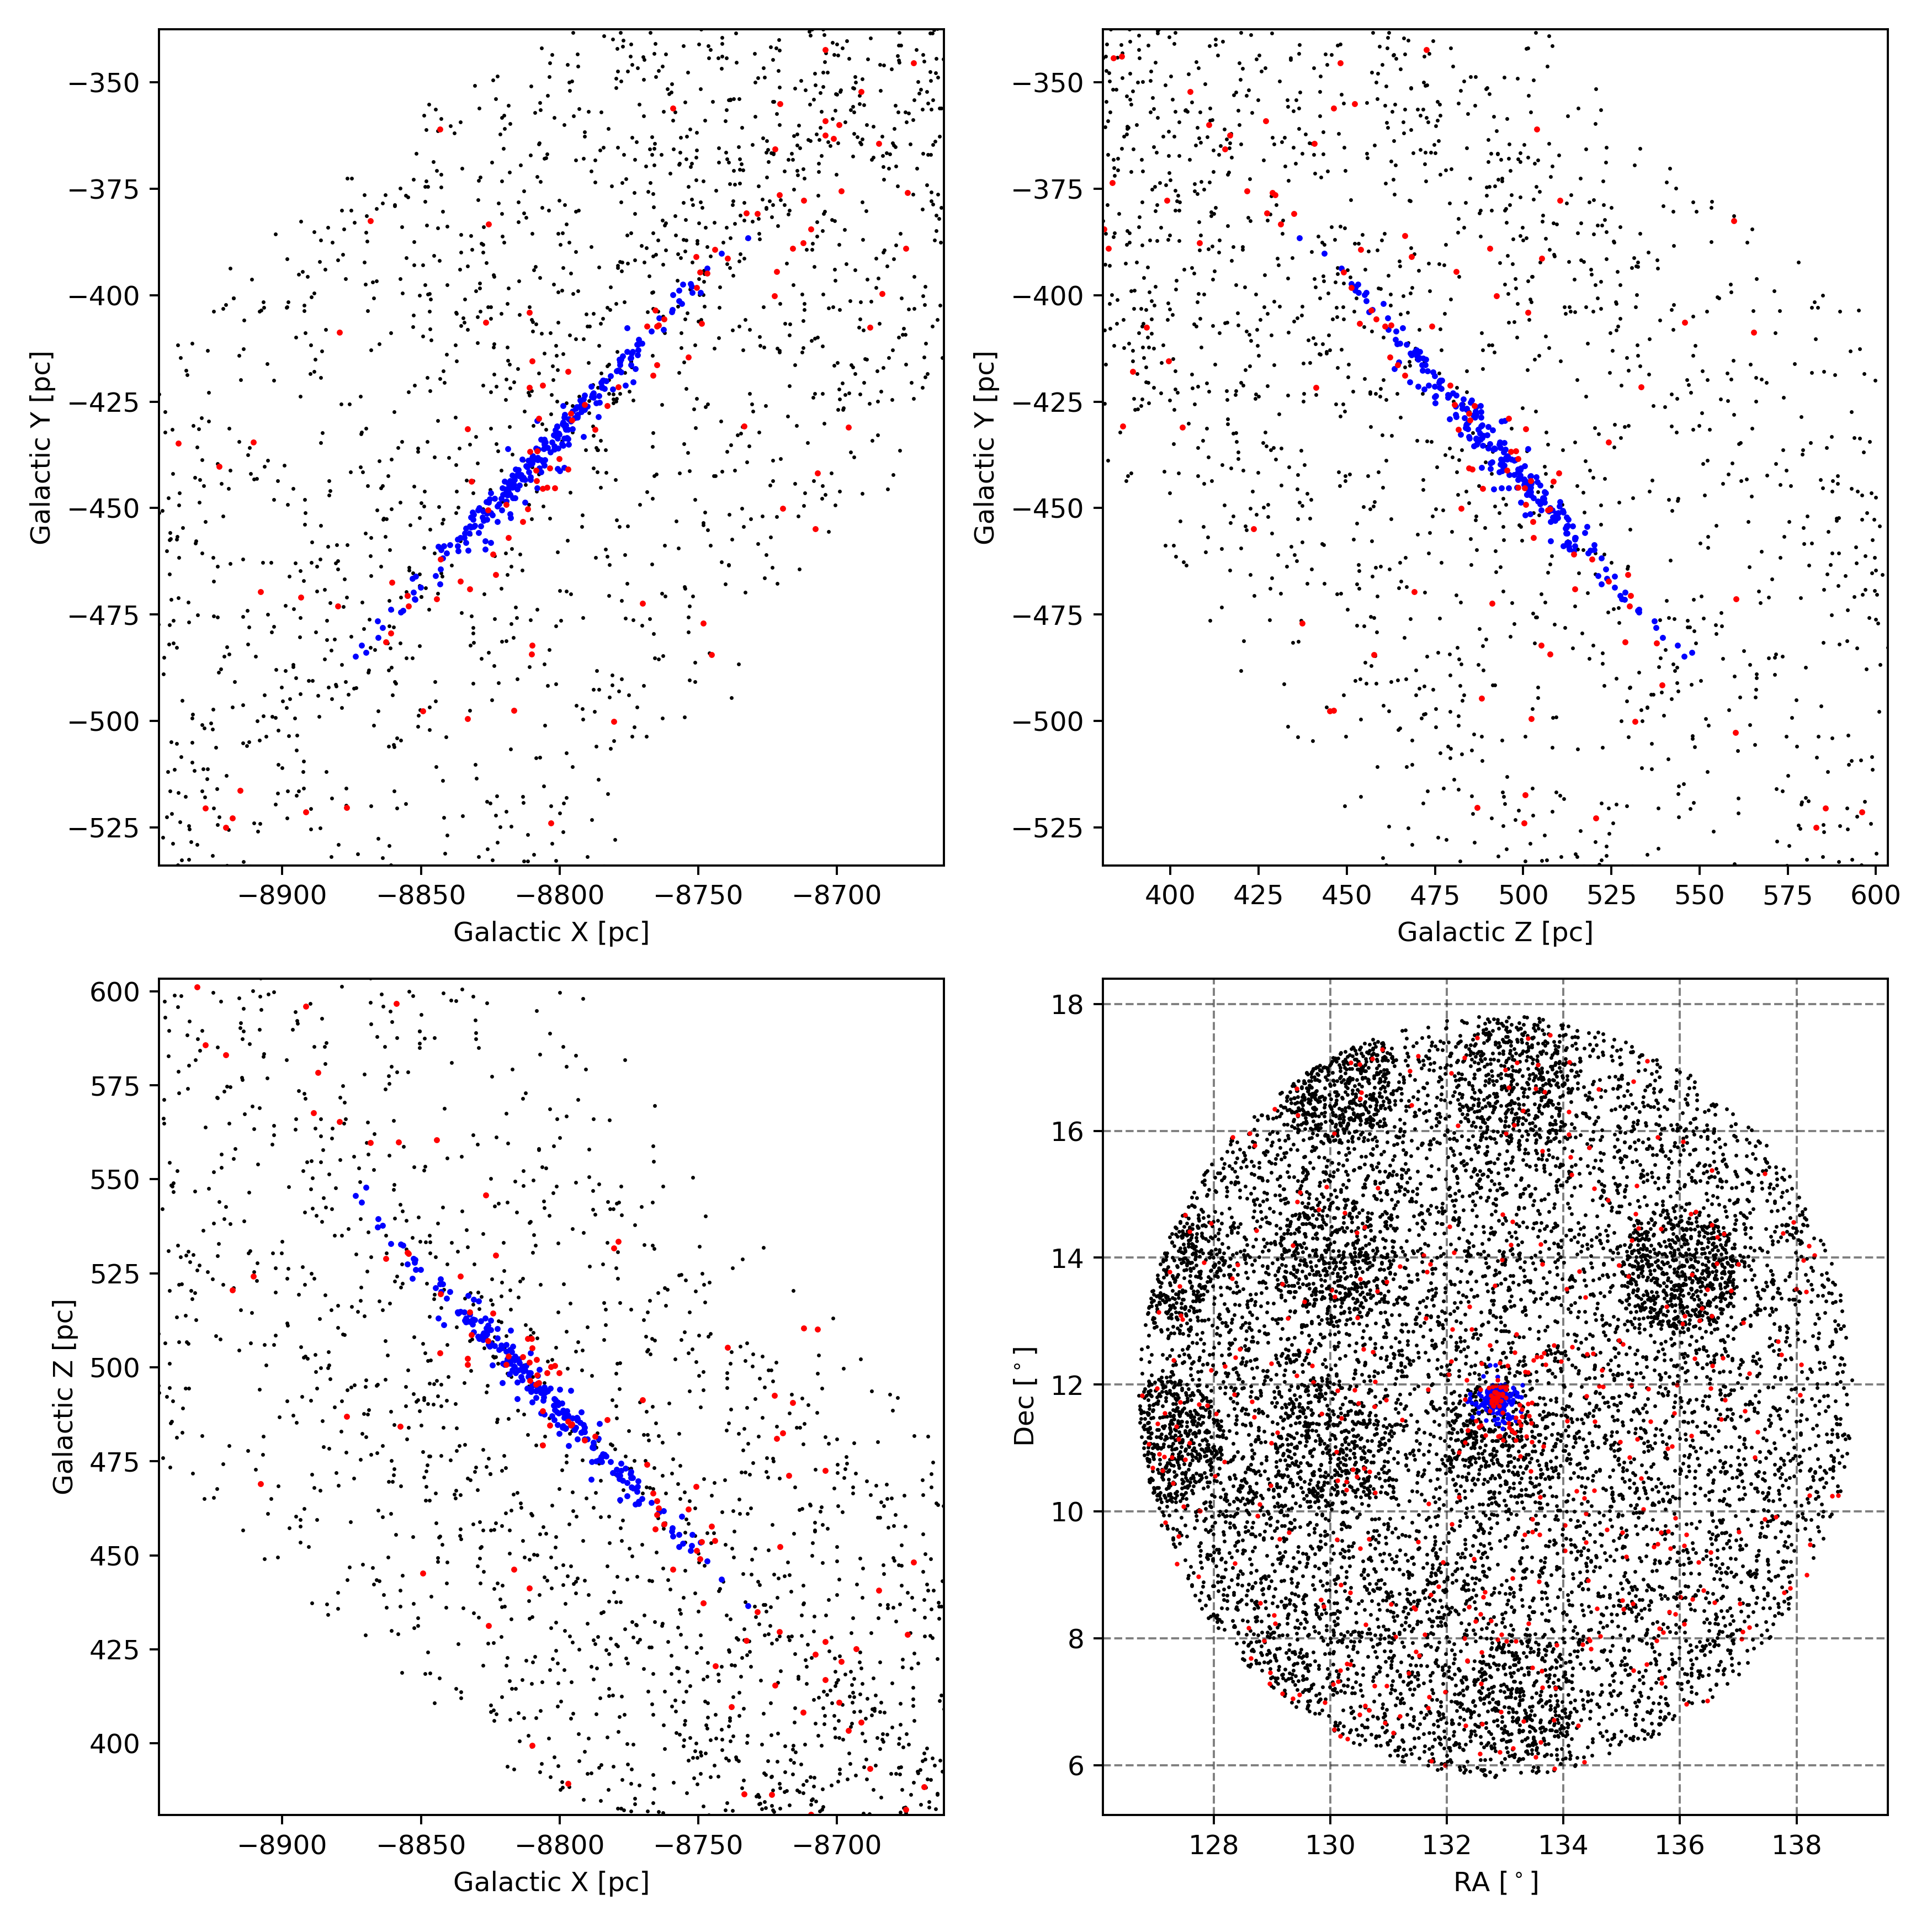
\includegraphics[width=\textwidth]{NGC_2682_possible_ejected-step1.png}
	\caption{Plots show the spatial distribution of the ejected candidates in red around the definite cluster members in blue. All other stars considered in the analysis are shown as black dots. First three panel shows the Galactic position of described cluster components. The denser circular patches of stars in the bottom right panel are not real stellar overdensities, but indicate regions where combined radial velocities of \G\ and \Gh\ are used. The example is given for the open cluster NGC 2682, which has the highest number of potentially ejected stars. Uncertainty of determined stellar distance is clearly evident as elongation of the main cluster body in the radial direction, away from the observers' position.}
	\label{fig:ejected_around_cluster}
\end{figure}

A much less energetic and more gradual mechanism that also influences the lifetime of an open cluster is tidal stripping of stars \cite{2006A&A...455L..17L}. It happens during clusters' journey through a more densely populated region such as galactic spiral arms. Tails reaching out of a cluster would, therefore, have elongated, probably slightly bent shape (not to be confused by the elongated cluster shape in Figure \ref{fig:ejected_around_cluster}), and not a spherical distribution as considered for ejection mechanism. In this section, we compare the chemical composition of known tidal structures (discovered in \Gs\ data by \citet{2019AA...627A...4R, 2019AA...627A.119C, 2019AA...621L...3M, 2019arXiv191206657Z}) of a few the \Gh\ open clusters with other previously defined and analysed structures. All of the aforementioned tidal structures were identified by different clustering methods of the same \G\ data and should, therefore, be in a sense similar to results of our orbital classification procedure. From the published tidal structures \cite{2019AA...627A...4R, 2019AA...627A.119C, 2019AA...621L...3M, 2019arXiv191206657Z}, we first removed all cluster members that were already identified by \citet{2018A&A...618A..93C} and consequently used in our procedure for the definition of clusters' chemical signature. In that way, our possibly ejected stars and tidal structures can be compared directly. Their overlap is shown in the fourth and fifth column of Table \ref{tab:cluster_stats_tails}. As the overlap between them is not zero, we can reliably say that we are all detecting similar kinematic structures using completely different approaches (but the same \G\ data). The identified structures therefore may or might not be related to neighbouring open cluster.

\begin{sidewaystable}
	\centering
	\caption{Statistics of detected stellar tidal structures around some of the clusters that were observed by the \Gh. The columns shown in the following order give information about: name of the analysed cluster, number of all stars found in the surrounding tidal structure, number of stars without cluster members, size of overlap between ejected and tail, number of unflagged \Gh\ observations among tidal structure, chemical similarity with parent open cluster, and reference source of the used data.}
	\begin{tabular}{l c c c c c r }
		\hline
		Cluster & Stars in & Without used & Common with & \Gh\ unflagged & Chemically & Membership\\
		& reference & cluster members & ejected & parameters (\% in & tagged & reference\\
		&  &  & (\% of ejected) & common with ejected) & (\% of valid) & \\
		\hline \hline
		Blanco 1   & 644 & 276 & 3 (50\%) & 7 (42.9\%) & 0 (0.0\%) & \citet{2019arXiv191206657Z} \\
		NGC 2632   & 1393 & 738 & 17 (22.1\%) & 25 (68\%) & 7 (28.0\%) & \citet{2019AA...627A...4R} \\
		NGC 2682   & 952 & 241 & 13 (14.4\%) & 18 (72.2\%) & 6 (33.3\%) & \citet{2019AA...627A.119C} \\
		Melotte 25 & 238 & 238 & 8 (30.8\%) & 57 (14.0\%) & 1 (1.8\%) & \citet{2019AA...621L...3M} \\
		\hline
	\end{tabular}
	\label{tab:cluster_stats_tails}
\end{sidewaystable}

Among randomly acquired The \Gh\ spectra, we observed some stars that where identified to belong to the kinematically discovered tidal structures around open clusters. If we consider only stars with unflagged the \Gh\ stellar parameters, the overlap between the sets is quite significant as more than 50\% of unflagged tail stars were also identified as possible ejected for every studied cluster. This significant overlap reduces probability of the tails having a completely different chemical signature than our selections, but at the same time confirms validity of our orbit tracing approach. 

For a tidal tail chemical tagging procedure, we used the same selection principle as previously described in Section \ref{sec:chem_ej_tag}. The results of the tagging experiment are presented in the last column of Table \ref{tab:cluster_stats_tails}. Majority of the tails have quite significant probability of being chemically similar to a nearby open cluster. 

\section{Summary and conclusions}
\label{sec:clusters_summary_conclusions}
Open clusters, as long known and widely studied stellar structures, still provide many opportunities for their exploration using new and improved information about their stellar components and neighbouring environment. In this chapter, we explored the latest multidimensional abundance data determined for stars observed in the scope of the \Gh\ survey, whose targets also consisted of stars in multiple open clusters. Combined with the \G\ kinematic information, a precise position, shape, and velocity of the cluster volume can be defined. We used the method of backward orbit integration to determine if any of the neighbouring stars could be kinematically traced back to the cluster and have the same chemical signature.

To verify that our orbital integration methodology gives sensible results, they were compared towards identified cluster tidal structures around the same open clusters. Given non zero overlap in all cases, we are confident that our structures are also related to the main cluster body.

Deepened analysis of field and cluster abundance patterns showed improvement in the quality of determined abundances (in comparison towards older \Gh\ releases), but at the same time revealed the pitfalls of blindly using massively determined abundances for blind chemical tagging experiments that are highly desired in the community of galactic archaeology. Identified problems can successfully be overcome by applying differential analysis, which in our case showed some encouraging success of using the \Gh\ abundance data as tracers of stellar birth signatures of individual stars. The tagging experiment showed that it was more likely that we could chemically tag a kinematically pre-selected star than a random nearby star. For a much firmer confirmation, we would require more observations as some of the cluster components were sparsely observed by the \Gh.

The explored methodology depends on the quality and correctness of the determined abundance trends. From the current data, it seems that identified abundance trends are valid only for an individual cluster as they can vary among them. This decreases possibility of preforming differential chemical tagging on larger, potentially galactic, scales.

To improve the parameters used in this chapter, we would have to analyse cluster members as a homogeneous structure that was formed at the same time. This adoption of formation time would force the use of a single isochrone and stellar age for all members, improving their determined \Logg, \Feh, and consequently also stellar surface chemical composition. Our first experiments with the mentioned analysis upgrade already show significant improvements in the stability of the trends and reduction of abundance scatter among cluster members.